\chapter{Grundlagen}\label{kap:grundlagen}

%####################  CHAPTER 1: Grundlagen  #################

Im vorliegenden Kapitel werden zunächst die Grundlagen 
des \Glspl{ml} mit \Glspl{nn}
beschrieben. Der zweite Abschnitt wird die in der 
Bilderkennung eingesetzen \Glsfirstplural{cnn} näher erläutern.
Im letzten Abschnitt wird die für die \Gls{inferenz} 
verwendete Hardware, der \textit{Neural Compute Stick 2}
von \textit{Intel} beschrieben.


%------------------- SECTION: Machine Learning ------------------

\section{Machine Learning}\label{sec:ml}

Beim \Gls{ml}, einem zentralen Begriff in der 
Künstlichen Intelligenz, geht es um die Erstellung von Algorithmen, 
die Zusammenhänge in 
großen Datenmengen erkennen und daraus Regeln ableiten können,
ohne explizit darauf programmiert worden zu sein.
Eine Form davon ist das \textit{Supervised Learning}, bei dem
das Programm neben den Inputdaten auch die zugehörigen Ausgaben,
in Form von Labels, erhält, um daraus 
Regeln für die Zusammenhänge zwischen Ein- und Ausgabedaten
abzuleiten.
Dadurch unterscheidet sich das Vorgehen wesentlich von der Programmierung 
eines klassischen Programms, bei dem die Regeln vorab definiert 
werden müssen, wie in Abbildung \ref{fig:classic_vs_ml}
veranschaulicht ist:
\vspace{0.5cm}

\begin{figure}[H]
    \centering
    
\tikzset{
    decision/.style={
        diamond,
        draw,
        text width=4em,
        text badly centered,
        inner sep=-1pt,
        node distance=8em
    },
    block/.style={
        rectangle,
        draw,
        text width=6em,
        %minimum widhth=6em,
        minimum height=3.5em,
        text centered,
        node distance=20em
    },
    arrow/.style={
        draw,
        >=latex,
        ->
    },
    textfeld/.style={
        %draw,
        text centered,
        node distance=1.5em
    }
}


\begin{tikzpicture}

    
    \node (system) [block] {Klassisches\\Programm};
    \node (system2) [block, right of=system] {ML\\Programm};

    \node [textfeld, left=of system.167] (inputs) {Daten};
    \node [textfeld, left=of system.193] (regeln) {Regeln};
    \node [textfeld, right=of system] (output) {Ausgaben};

    \node [textfeld, left=of system2.167] (inputs2) {Daten};
    \node [textfeld, left=of system2.193] (output2) {Ausgaben};
    \node [textfeld, right=of system2] (regeln2) {Regeln};
    
    \draw[arrow] (inputs) -- (system.167);
    \draw[arrow] (regeln) -- (system.193);
    \draw[arrow] (system) -- (output);
    
    \draw[arrow] (inputs2) -- (system2.167);
    \draw[arrow] (output2) -- (system2.193);
    \draw[arrow] (system2) -- (regeln2);
    

\end{tikzpicture}

    \caption{Vergleich herkömmliche und Machine-Learning-Programmierung}
    \label{fig:classic_vs_ml}
\end{figure}
\vspace{0.5cm}

Das Ableiten der Regeln erfolgt beim \Gls{ml} in einem 
iterativen Prozess, welcher als Training bezeichnet wird.
Dabei werden die Zusammenhänge zwischen Ein- und Ausgabedaten 
als mathematische Funktion betrachtet, die numerisch an die richtigen Werte
angenähert wird.

Handelt es sich um einen linearen Zusammenhang der 
Daten spricht man von einer \textit{Regression}, 
wohingegen bei einer Kategorisierung von diskreten 
Werten von einer \textit{Klassifikation} gesprochen wird.

Weitere Formen neben dem \textit{Supervised Learning} sind das 
\textit{Unsupervised Learning}, bei dem das Programm keine Labels 
erhält, sondern diese durch das Training selber finden 
soll, oder das \textit{Reinfocement Learning}, bei dem das Programm 
Rückmeldung zu seinen Aktionen bekommt und dadurch sein Vorgehen
optimiert.

In dieser Bachelorarbeit wurde das \textit{Supervised Learning}
verwendet, da sich damit die Aufgabe zur Erkennung und Klassifizierung 
von Objekten am besten realisieren lässt.

%------------------- SECTION: Neuronale Netze -------------------

%\newpage
\subsection{Künstliche Neuronale Netze} \label{subsec:nn}

Für die Verarbeitung komplexer Inputdaten,
wie beispielsweise Bilder, bei denen 
die einzelnen Pixelwerte die Eingaben und der Inhalt des Bildes die 
gesuchte Ausgabe darstellen, eignen sich in besonderer Weise 
die \Glspl{nn}.
Diese sind eine Teilgebiet des \Glspl{ml} und bestehen
aus einer Vielzahl an programmatisch erzeugten künstlichen Neuronen,
die in Schichten angeordnet miteinander verbunden sind.

Durch unterschiedlich starke Gewichtungen der einzelnen
Verbindungen, welche als Gewichte bezeichnet werden, 
können zu gegebenen Eingaben die richtigen Ausgaben gefunden werden,
wie in Abbildung \ref{fig:nn} schematisch dargestellt ist.
\vspace{1cm}

\begin{figure}[H]
    \centering
    \def\svgwidth{0.85\columnwidth}
    %\footnotesize
    \begin{neuralnetwork}[height=1]
    \newcommand{\nodetextclear}[2]{}
    \newcommand{\nodetexth}[2]{$h_#2$}
    \newcommand{\nodetextx}[2]{$x_#2$}
    \newcommand{\nodetexty}[2]{$y_#2$}
    \inputlayer[count=3, bias=false, title=Input\\layer, text=\nodetextx]
    \hiddenlayer[count=4, bias=false, title=Hidden\\layer, text=\nodetexth] \linklayers
    \outputlayer[count=2, title=Output\\layer, text=\nodetexty] \linklayers
\end{neuralnetwork}
    \caption{Vereinfachte Darstellung eines Künstlichen 
    Neuronalen Netzes}
    \label{fig:nn}
\end{figure}
\vspace{1cm}

Die richtigen Einstellungen der Gewichte erfolgt dabei
in einem iterativen Trainingsprozess, der aus folgenden 
drei Schritten besteht und in Abbildung \ref{fig:train}
schematisch dargestellt ist. 

\begin{itemize}
    \item \textit{Forward Pass} Für die Inputdaten anhand
            aktueller Gewichte eine Vorhersage für die Ausgabe treffen
    \item \textit{Fehlerbestimmung} Abweichung der gemachten Vorhersage
             zum tatsächlichen Wert (Labels) über eine Fehlerfunktion berechnen
    \item \textit{Backpropagation} Minimierung der
            Abweichung durch Anpassung der Gewichte (Optimierer)
\end{itemize}

\vspace{1cm}
\begin{figure}[H]
    \centering
    
\tikzstyle{process} = [rectangle, fill=blue!20, minimum width=2.5cm, minimum height=1cm, text centered, draw=black]
\tikzstyle{arrow} = [thick,->,>=stealth]

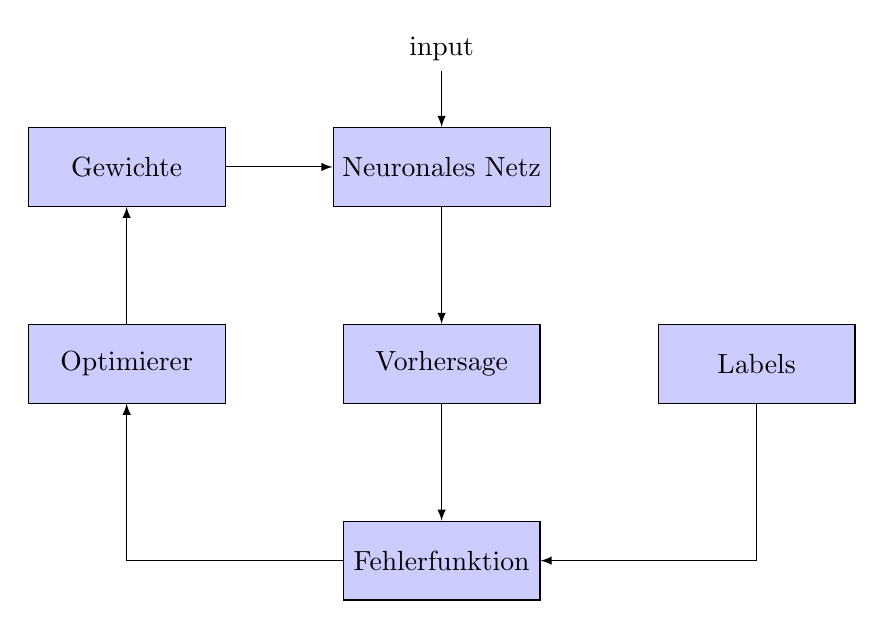
\begin{tikzpicture}[node distance=1.6cm]

  \begin{scope}[node distance=2.5cm]
    \node (nn)      [process]                   {Neuronales Netz};
    \node (pred)      [process, below of=nn]      {Vorhersage};
    \node (loss)      [process, below of=pred]      {Fehlerfunktion};
    
  \end{scope}
  
  \begin{scope}[node distance=4cm]
    \node (opt) [process, left of=pred]      {Optimierer};
    \node (weights)  [process, left of=nn] {Gewichte};
    \node (labels)   [process, right of=pred]  {Labels};
  \end{scope}

  \node (input) at (0,1.5) {input};

  \draw[arrow] (input) -- (nn);

  \draw[arrow] (nn) -- (pred);
  \draw[arrow] (pred) -- (loss);

  \draw[arrow] (labels) |- (loss);
  \draw[arrow] (loss) -| (opt);

  \draw[arrow] (opt) -- (weights);
  \draw[arrow] (weights) -- (nn);
  
    
\end{tikzpicture}

    \caption{Schematischer Trainingsablauf eines Neuronalen Netzes}
    \label{fig:train}
\end{figure}
\vspace{1cm}


Durch mehrfaches Durchlaufen dieser Schritte 
kann die Fehlerfunktion soweit minimiert werden, dass 
das Modell auch für neue, unbekannte Inputdaten 
richtige Vorhersagen treffen kann.

Die Funktionsweisen der drei Schritte 
werden im Folgenden näher erläutert.

\subsubsection{Forward Pass}
Im \textit{Forward Pass} werden die Eingabewerte, welche an der 
ersten Schicht aus Neuronen anliegen, durch alle Schichten hindurch 
gereicht, um in der Ausgabeschicht
das gesuchte Ergebnis zu liefern.
Dabei erhält jedes Neuron die mit den Parametern $w_{i}$ gewichteten
Ausgabewerte aller Neuronen der vorherigen Schicht und summiert diese
zusammen mit einem konstanten Bias Wert $b$ als Offset auf.

Mithilfe einer Aktivierungsfunktion wird der Wert, wie 
in Abbildung \ref{fig:neuron} dargestellt, auf
einen bestimmten Bereich skaliert.


\vspace{1cm}
\begin{figure}[H]
    \centering
    \begin{tikzpicture}[
    % define styles    
    init/.style={ 
         draw, 
         circle, 
         inner sep=2pt,
         font=\Huge,
         join = by -latex
    },
    squa_draw/.style={ 
        draw,
        font=\Large,
        join = by -latex
    },
    squa/.style={ 
        font=\Large,
        join = by -latex
    }
]
% Top chain x1 to w1
\begin{scope}[start chain=1]
    \node[on chain=1] at (0,1.5cm)  (x1) {$x_1$};
    \node[on chain=1,join=by o-latex] (w1) {$w_1$};
\end{scope}
% Middle chain x2 to output
\begin{scope}[start chain=2]
    \node[on chain=2] (x2) {$x_2$};
    \node[on chain=2,join=by o-latex] {$w_2$};
    \node[on chain=2,init] (sigma) {$\displaystyle\Sigma$};
    \node[on chain=2,squa_draw,label=below:{\parbox{2cm}{\centering Aktivierungs-funktion}}]   {$g(z)$};
    \node[on chain=2,squa,label=below:Output,join=by -latex] {$y_{out}$};
\end{scope}
% Bottom chain x3 to w3
\begin{scope}[start chain=3]
    \node[on chain=3,label=below:Inputs] at (0,-1.5cm) 
    (x3) {$x_3$};
    \node[on chain=3,label=below:Gewichte,join=by o-latex]
    (w3) {$w_3$};
\end{scope}
% Bias
\node[label=above:\parbox{2cm}{\centering Bias \\ $b$}] at (sigma|-w1) (b) {};
% Arrows joining w1, w3 and b to sigma
\draw[-latex] (w1) -- (sigma);
\draw[-latex] (w3) -- (sigma);
\draw[o-latex] (b) -- (sigma);

\end{tikzpicture}

% von https://medium.com/momenton/typesetting-neural-network-diagrams-with-tex-4920b6b9fc19
    \caption{Berechnungen an einem einzelnen Neuron}
    \label{fig:neuron}
\end{figure}
\vspace{1cm}

Um diesen Vorgang für eine gesamte Schicht, bestehend aus 
einer Vielzahl an Neuronen, zu berechnen, werden die Schichten 
als Vektoren $x$ und die Gewichte als Matrizen $W$ dargestellt.

Durch Bilden der Matrixmultiplikation zwischen $x$ und $W$,
 wie Gleichung \ref{eq:forward} zeigt,
erhält man den \textit{Forward Pass} von einer Schicht zur nächsten.
\vspace{0.5cm}

\begin{equation}
    \label{eq:forward}
    z = W^{T}x+b
\end{equation}
\vspace{0.5cm}

Der resultierende Vektor $z$ wird dann elementweise
einer nichtlinearen Aktivierungsfunktion $g(z)$ übergeben.

Bei dieser handelt es sich für die mittleren Schichten 
(die sogenannten \textit{Hidden Layer})
meistens um die in Abbildung \ref{plot:relu} dargestellte
Funktion \textit{ReLU}, welche positive Werte beibehält und negative 
Werte auf 0 setzt.

In der letzten Schicht, welche die Wahrscheinlichkeiten 
für mögliche Ausgaben enthält, wird eine Aktivierungsfunktion
verwendet, die den Wert zwischen 0 und 1 skaliert.
Dabei wird für eine binäre Klassifikation die 
in Abbildung \ref{plot:sigmoid} dargestellte \textit{Sigmoidfunktion}
verwendet, welche die Werte s-förmig auf einen Bereich zwischen 
0 und 1 skaliert.

Für eine kategorische Klassifikation 
mit mehr als zwei möglichen Ausgabewerten
wird die in Gleichung 
\ref{eq:softmax} dargestellte \textit{Softmax-Funktion} 
verwendet, die eine
Wahrscheinlichkeitsverteilung über alle Werte
der Ausgabeschicht generiert.

\begin{equation}
    \label{eq:softmax}
    g(z_{i}) = \frac{e^{z_{i}}}{\sum_{j} e^{z_{j}}}
\end{equation}
%\newpage
%\vspace{1cm}
\begin{minipage}{0.5\textwidth}
    \centering
    \begin{equation*}
        \label{eq:relu}
        g(z) = max\{0,z\}
    \end{equation*}
\end{minipage}
\vspace{1cm}
\begin{minipage}{0.5\textwidth}
    \centering
    \begin{equation*}
        \label{eq:sidmoid}
        g(z) = \frac{1}{1 + e^{-z}}
    \end{equation*}    
\end{minipage}
\begin{minipage}{0.5\textwidth}
    \centering
    \begin{tikzpicture}[scale=0.6]
    \begin{axis}
        %scale only axis=true,
        [
            scale only axis=true,
            width=0.8\textwidth,
            height=5cm,
            axis x line=middle,
            axis y line=center,
            tick align=outside
        ]
        
        \addplot
        [
            blue,
            mark=none,
            smooth,
            domain=-3:6
        ] 
        (x,{(x>=0)*x});

	\end{axis}
\end{tikzpicture}
    \captionof{figure}{ReLU} 
    \label{plot:relu}
\end{minipage}
\begin{minipage}{0.5\textwidth}
    \centering
    \begin{tikzpicture}[scale=0.8]
    \begin{axis}
        %scale only axis=true,
        [
            scale only axis=true,
            width=\textwidth,
            height=5cm,
            % xmin=-6,
            % xmax=6,
            axis x line=middle,
            axis y line=center,
            tick align=outside
        ]
        
        \addplot
        [
            blue,
            mark=none,
            smooth,
            domain=-6:6
        ] 
        (x,{1/(1+exp(-x))});

	\end{axis}
\end{tikzpicture}
    \captionof{figure}{Sigmoidfunktion} 
    \label{plot:sigmoid}
\end{minipage}
\vspace{1cm}


\subsubsection{Fehlerbestimmung}
Die Abweichung des geschätzten Wertes, der an den
Neuronen der letzten Schicht anliegt, zum tatsächlichen Wert
wird mithilfe einer geeigneten Fehlerfunktion (Loss-Funktion)
ermittelt.
Ein Regressionsmodell verwendet hierfür oft 
den absoluten oder quadratischen Abstand der beiden 
Werte, wohingegen für Klassifikationsmodelle meistens 
eine logarithmische Funktion verwendet wird.
In Gleichung \ref{eq:crossentropy} ist die logarithmische
Loss-Funktion \textit{Cross entropy} für eine binäre
Klassifikation dargestellt.
Durch den Logarithmus wird der Loss-Wert um so größer,
je weiter die Schätzung $y$ vom 
tatsächlichen Wert $\hat{y}$ abweicht.
\vspace{0.5cm}

\begin{equation}
    \label{eq:crossentropy}
    L = \hat{y}log(y) + (1 - \hat{y})log(1 - y)
\end{equation}
\vspace{0.5cm}


\subsubsection{Backpropagation}

Die Anpassung der Gewichte zur Minimierung der Loss-Funktion 
kann durch Berechnung des Gradienten der Loss-Funktion erfolgen.

Dafür wird die Loss-Funktion $L$ für jede Schicht partiell
mithilfe der Kettenregel nach den Gewichten $w$ der jeweiligen
Schicht abgeleitet, siehe Gleichung \ref{eq:backprop}.

Mit den ermittelten Gradienten werden
dann die Gewichte 
mit einer Schrittweite $\eta$ angepasst, siehe 
Gleichung \ref{eq:update_wieghts}.
\vspace{0.5cm}

\begin{equation}
    \label{eq:backprop}
    \frac{\partial L}{\partial w} = \frac{\partial L}{\partial z}\frac{\partial z}{\partial w}
\end{equation}
\vspace{0.5cm}
\begin{equation}
    \label{eq:update_wieghts}
    w  \leftarrow w - \eta \frac{\partial L}{\partial w}
\end{equation}
\vspace{1cm}



%------------------- SUBSECTION: Validierung -------------------
\subsection{Validierung und Overfitting}\label{subsec:validation}

Um überprüfen zu können, ob und wie gut ein Modell die Zusammenhänge
in den Trainingsdaten generalisiert hat und damit auch für neue
 Daten anwendbar ist, wird der Datensatz in einen Trainings- und
einen Testdatensatz aufgeteilt.

Die Abweichung von den tatsächlichen Werten wird während
des Trainings für beide Datensätze 
berechnet, die Korrektur der Gewichte mittels
\textit{Backpropagation} erfolgt jedoch nur anhand
der Trainingsdaten.

Indem beide Loss-Werte als Funktionen in Abhängigkeit 
der Iterationen geplottet werden, kann eine Überanpassung
des Modells an die Trainingsdaten festgestellt werden.

Dabei handelt es sich um das sogenannte \textit{\Gls{overfitting}},
was daran zu erkennen ist, dass sich nur noch der Loss-Wert der 
Trainingsdaten verringert und der Wert der Testdaten 
gleich bleibt oder sich wie in Abbildung \ref{fig:overfitting}
dargestellt, wieder verschlechtert.
\vspace{1cm}

\begin{figure}[H]
    \centering
    \def\svgwidth{0.5\textwidth}
    \input{Bilder/overfitting.pdf_tex}
    \caption{Overfitting dargestellt anhand der Loss-Kurven}
    \label{fig:overfitting}
\end{figure}
\vspace{1cm}

Gründe für das \textit{\Gls{overfitting}} können sein,
dass zu wenig Trainingsdaten
verwendet wurden oder ein für den Anwendungsfall 
zu komplexes Modell gewählt wurde.

Durch die große Anzahl an Parametern eines zu komplexen Modells
hat dieses die Möglichkeit, sich an jeden Trainingsdatenpunkt einzeln
anzupassen, sodass keine generalisierbaren 
Aussagen für neue Datenpunkte mehr getroffen werden können.

Der andere Extremfall ist das \textit{Underfitting}, 
bei dem das Modell aufgrund zu weniger Parameter nicht die 
Möglichkeit hat, sich an die Trainingsdaten anzunähern.

Die Plots in Abbildung \ref{fig:over_under_fit} veranschaulichen 
die drei Fälle anhand einer polynomialen Funktion, die sich 
mit unterschiedlich hohem Grad an gegebene Datenpunkte 
annähern soll.

\vspace{1cm}
\begin{figure}[H]
    \centering
    \def\svgwidth{\textwidth}
    \input{Bilder/over_under_fit.pdf_tex}
    \caption{Annäherung unterschiedlich komplexer
    Funktionen an gegebene 
        Datenpunkte}
    \label{fig:over_under_fit}
\end{figure}
\vspace{1cm}

Das Auftreten von \textit{\Gls{overfitting}} kann entweder durch 
Verwendung einer größeren Anzahl von Trainingsdaten vermieden werden 
oder mit einer der folgenden Techniken:


\subsubsection{Augmentierung}

\textit{Augmentierung} der Daten ist eine effektive Technik 
zur Reduzierung von \textit{\Gls{overfitting}}, bei der künstlich,
aus den vorhandenen Daten, zusätzliche Daten generiert werden. 
Im Fall der Bilderkennung werden hierbei 
die Inputbilder leicht abgeändert, indem z.B. geometrische 
Transformationen oder sonstige Manipulationen der Pixelwerte 
vorgenommen werden.


\subsubsection{Regularisierung}

Bei der \textit{Regularisierung} wird der Loss-Funktion,
als weiterer Term, eine Aufsummierung aller Gewichte
hinzugefügt.

Die Minimierung der Loss-Funktion hat dann den Effekt, dass
die Gewichte möglichst 
kleine Werte behalten, wodurch das Modell weniger
Möglichkeiten zur Überanpassung hat.

Dabei wird zwischen der \textit{L1 Regularisierung}
mit einer absoluten und der \textit{L2 Regularisierung} mit einer 
quadratischen Aufsummierung der
Gewichte unterschieden, wie in Gleichung \ref{eq:regularization}
dargestellt.

\begin{equation}
    \label{eq:regularization}
    J = L + \lambda \sum_{i} w_{i}^{2}
\end{equation}


\subsubsection{Dropout}
\textit{Dropout} ist eine Technik, bei der in einigen Schichten 
mit einer bestimmten Wahrscheinlichkeit Werte von 
Neuronen auf 0 gesetzt werden.
Dadurch wird das Modell gezwungen, alternative
Gewichtsanpassungen zu finden.

\begin{figure}[H]
    \centering
    \includegraphics[width=0.6\textwidth]{dropout.png}
    \caption{Funktionsprinzip Dropout 
    \cite{JMLR:v15:srivastava14a}}
    \label{fig:dropout}
\end{figure}

\subsubsection{Early Stopping}
Beim \textit{Early Stopping} wird das Training abgebrochen, 
bevor \textit{\Gls{overfitting}} stattfinden kann.
Das ist, wie in Abbildung \ref{fig:overfitting}
markiert, durch das Minimum der Loss-Kurve der Testdaten 
definiert.


%------------------- SUBSECTION: ML Frameworks ---------------
\subsection{Machine Learning Frameworks}

\textit{Machine-Learning}-Algorithmen beinhalten eine
Vielzahl an komplexen Berechnungsschritten und Parametern.
Um diese nicht jedesmal von Grund auf neu implementieren zu müssen,
bieten \Glspl{framework} eine einfache Möglichkeit, 
aufbauend auf vorimplementierten Programmkomponenten,
eigene Modelle zu konstruieren.

Einige der bekannten Open Source \Glspl{framework} sind
\textit{TensorFlow, Caffe, Torch, Kaldi} oder \textit{Scikit-Learn}.

Für diese Bachelorarbeit wurde \textit{TensorFlow} verwendet,
ein von Google stammendes \Gls{framework},
welches aufgrund seiner hohen Flexibilität häufig in
der Forschung verwendet wird.



%---------------- SUBSECTION: Convolutional ----------------
\section{Convolutional Neural Networks}\label{subsec:cnn}

\Glsfirstplural{cnn} erweitern die in Abschnitt \ref{subsec:nn} beschriebenen
Künstlichen Neuronalen Netze um zusätzliche Schichten,
die vor der eigentlichen Klassifikation ausgeführt werden
und Merkmale aus den Inputdaten herausextrahieren.
Diese Schichten erhalten die Inputdaten als
zweidimensionale Matrix und führen darauf eine 
mathematische \Gls{faltung} aus.
\Glspl{cnn} kommen größtenteils in der Bilderkennung zum 
Einsatz, ein weiteres Anwendungsgebiete ist 
z.B. die Spracherkennung.

Anstatt dass alle Neuronen zweier benachbarter Schichten 
durch gewichtete Parameter miteinander verbunden sind, 
stellen kleinere, sogenannte Filtermatrizen, die 
Parameter dar.
Diese werden zeilenweise über das Inputbild 
geschoben, wobei an jeder Stelle eine mathematische 
\Gls{faltung} mit dem überlappten Bereich des Inputs 
durchgeführt wird. In Abbildung \ref{fig:faltung}
ist dieser Vorgang zur Veranschaulichung dargestellt.
\vspace{1cm}

\begin{figure}[H]
    \centering
    \begin{minipage}{0.49\textwidth}
        \centering
        \includegraphics[width=0.9\textwidth]{convolution.png}
    \end{minipage}
    \begin{minipage}{0.49\textwidth}
        \centering
        \includegraphics[width=0.9\textwidth]
        {convolution-layer-a.png}
    \end{minipage}  
    \caption{\Gls{faltung} des Inputs mit einer Filtermatrix
    \cite{faltung}
    \cite{faltung2}}
    \label{fig:faltung}
\end{figure}
\vspace{1cm}


Jedes \Gls{faltung}sergebnis entspricht einem Wert
in der nächsten Schicht, welche die Korrelation 
von Filter Matrix und Inputbild angibt.
So werden in den Filtern definierte Muster, wie 
beispielsweise vertikale Linien, 
aus dem Inputbild herausextrahiert und in 
den Folgeschichten in den sogenannten
\textit{\Glspl{featuremap}} abgebildet.

\vspace{1cm}

\begin{equation}
    \label{eq:faltung}
    \begin{pmatrix}
        10 & 10 & 10 & 0 & 0 & 0\\
        10 & 10 & 10 & 0 & 0 & 0\\
        10 & 10 & 10 & 0 & 0 & 0\\
        10 & 10 & 10 & 0 & 0 & 0\\
        10 & 10 & 10 & 0 & 0 & 0\\
        10 & 10 & 10 & 0 & 0 & 0
    \end{pmatrix}
    \times
    \begin{pmatrix}
        1 & 0 & -1\\
        1 & 0 & -1\\
        1 & 0 & -1
    \end{pmatrix}
    = 
    \begin{pmatrix}
        0 & 30 & 30 & 0\\
        0 & 30 & 30 & 0\\
        0 & 30 & 30 & 0\\
        0 & 30 & 30 & 0
    \end{pmatrix}
\end{equation}
\vspace{0.5cm}
\begin{figure}[H]
    \centering
    \def\svgwidth{0.6\textwidth}
    \input{Bilder/convolution_graphical_all.pdf_tex}
    \caption{\Gls{faltung} des Inputs mit einer
    Filtermatrix zur Erkennung vertikaler Linien}
    \label{fig:faltung3}
\end{figure}

In Gleichung \ref{eq:faltung} ist beispielhaft die \Gls{faltung} 
eines Inputbildes mit einem Filter zur Erkennung 
vertikaler Linien dargestellt. Da pro Zeile 
vier \Glspl{faltung} angewendet werden, entsteht 
eine $4\times4$ Matrix. Soll die Ausgangsgröße 
(hier $6\times6$) beibehalten werden, kann
\textit{\Gls{zeropadding}} verwendet werden.
Durch die \Gls{faltung} entsteht eine räumliche 
Invarianz für das zu erkennende Objekt im 
Inputbild.

Den \textit{Convolutional Layern} folgen meist
\textit{Pooling Layer} zum \Gls{downsampling},
und eine ReLU Aktivierungsfunktion. Eine solche 
Abfolge wird als \textit{Convolutional-Block}
bezeichnet.
Beim Pooling wird eine bestimmte Anzahl von Werten 
zusammengefasst, indem entweder das Maximum oder der 
Mittelwert dieser Werte verwendet wird.
Durch Hintereinanderschaltung mehrerer solcher
\textit{Convolutional-Blöcke} lassen sich
mit jeder weiteren Schicht auch komplexere 
Muster aus dem Inputbild herausextrahieren.

Die Features des letzten \textit{Convolutional Layers}
werden dann einem \textit{Fully Connected Layer}
zur Klassifikation übergeben.
In Abbildung \ref{fig:lenet} ist die beschriebene 
Struktur anhand des ersten, von Yann LeCun 
entworfenen \Gls{cnn}, dargestellt.
\vspace{1cm}

\begin{figure}[H]
    \centering
    \includegraphics[width=\columnwidth]{lenet.png}
    \caption{LeNet-5 Architektur
    \cite{lecunGradientBasedLearningApplied1998}}
    \label{fig:lenet}
\end{figure}
\vspace{1cm}

Ein wesentlicher Vorteil gegenüber einem reinen 
\textit{Feedforward Network} ist, dass 
durch die Verwendung von Filtermatrizen 
weniger Parameter verwendet werden müssen
und somit ein geringerer Rechenaufwand notwendig ist.
Die Werte der Filtermatrizen, welche die zu 
extrahierenden Muster repräsentieren, 
werden über die \textit{Backpropagation} gelernt.

Da die Merkmale insbesondere in den vorderen 
\textit{Convolutional Layern} für die meisten 
Klassen sehr ähnlich sind,
werden häufig Modelle mit vortrainierten Filtern 
verwendet, was als \textit{Transfer Learning}
bezeichnet wird.
Dadurch müssen die Gewichte nur noch geringfügig 
an den eigenen Datensatz angepasst werden.



\subsection{Architekturen}\label{subsubsec:architectures}

Nachdem 1998 das erste \Gls{cnn} (Abbildung \ref{fig:lenet})
 von Yann LeCun 
\cite{lecunGradientBasedLearningApplied1998} 
vorgestellt wurde, gab es eine Vielzahl 
von Weiterentwicklungen, die genauere und 
effizientere Modelle hervorbrachten.

Gemessen und verglichen werden die Ergebnisse häufig 
im Rahmen eines jährlich stattfindenden Software-Wettbewerbs, 
der \textit{Large Scale Visual Recognition Challenge (ILSVRC)}
\cite{ILSVRC15}.

Namhafte Modelle, welche den Wettbewerb in den letzten 
Jahren gewinnen konnten, sind unter \cite{stanfordConvNetList}
zu finden und im Folgenden aufgelistet.


\begin{itemize}
    \item \textbf{AlexNet}, (2012), von Alex Krizhevsky 
        \cite{krizhevskyImageNetClassificationDeep2017b} besitzt eine 
        ähnliche Struktur wie LeCuns \textit{LeNet},
        ist jedoch tiefer und besitzt mehrere \textit{Convolutional
         Layer} am Stück hintereinander,
        wodurch die Genauigkeit erhöht wurde.

    \item \textbf{ZF Net}, (2013), von Matthew Zeiler and Rob Fergus,
        \cite{zeilerVisualizingUnderstandingConvolutional2013}
        konnte das \textit{AlexNet} durch eine Vergrößerung der 
        mittleren \textit{Convolutional Layer}
        und eine Verkleinerung der Filter in den vorderen
        Schichten weiter optimieren.

    \item \textbf{VGGNet}, (2014), von Karen Simonyan and Andrew Zisserman.
        \cite{simonyanVeryDeepConvolutional2015}.
        Dieses Modell zeigte, dass ein tieferes Netz
         (16 bis 19 \textit{Convolutional Layer})
        mit reduzierter Filtergröße ($3\times3$) bessere
        Ergebnisse erzielt.    

    \item \textbf{GoogleLeNet}, (2014), auch bekannt als \textit{Inception},
        von Szegedy et al \cite{szegedyGoingDeeperConvolutions2014},
        konnte mit den \textit{Inception-Modulen},
        welche im Folgenden genauer erläutert werden, die Zahl der 
        Parameter und dadurch den Rechenaufwand deutlich verringern.

    \item \textbf{ResNet}, (2015), von Kaiming He et al 
        \cite{heDeepResidualLearning2015}, enthält 
        als Erweiterung die \textit{Residual Blöcke}, in denen auf
        das Ergebnis eines Blocks zusätzlich der unveränderte
        Inputwert addiert wird.
\end{itemize}


Im Folgenden werden die in der Bachelorarbeit verwendeten 
\Gls{cnn}-Modelle genauer beschrieben.

\subsubsection{GoogleLeNet (Inception)}

Die Entwicklung der \Gls{cnn} Architekturen hat gezeigt,
dass sich durch Hinzufügen weiterer Schichten, sowie
durch die Verwendung einer größeren Anzahl von Neuronen je Schicht 
die Genauigkeit verbessern lässt.
Das bringt jedoch auch die Nachteile eines 
größeren Rechenaufwands sowie der erhöhten 
Gefahr des \Glspl{overfitting} mit sich.

Das in \cite{szegedyGoingDeeperConvolutions2014} 
vorgestellte \textit{GoogleLeNet} hat mit den in 
Abbildung \ref{fig:incept_modul} dargestellten
\textit{Inception-Modulen} einen neuen, 
effizienteren Ansatz gefunden, die 
Komplexität und damit die Genauigkeit eines 
\Glspl{cnn} zu erhöhen.

Die Module bestehen aus parallel ausgeführten 
\textit{Convolutional Layern} mit den 
unterschiedlichen Filtergrößen $1\times1$,
 $3\times3$ und $5\times5$, welche 
am Ende des Moduls über eine \textit{Filter 
concatenation} wieder zusammengeführt werden.
Zur Dimensionsreduktion werden, wie in 
Abbildung \ref{fig:incept_modul} dargestellt,
diesen Filtern noch $1\times1$ Filter vorgeschaltet.
Durch die \textit{Inception-Module} erzielt das Modell 
mit deutlich weniger 
Parametern die gleichen Ergebnisse
wie ein Modell ohne die Module mit entsprechend mehr Parametern.
Ein weiterer Vorteil liegt darin, dass durch die 
unterschiedlichen Filtergrößen Merkmale 
unterschiedlicher Skalierungen besser gefunden 
werden können.

Um die Effizienz weiter zu steigern, wurden in 
der zweiten Version des \textit{GoogleLeNet}, beschrieben in
\cite{szegedyRethinkingInceptionArchitecture2015},
neben anderen Verbesserungen, die 
$5\times5$ Filter jeweils durch zwei $3\times3$ Filter 
ersetzt, was in Abbildung \ref{fig:incept_modul2}
dargestellt ist.
\vspace{1cm}

\begin{minipage}{0.45\textwidth}
    \centering
    \input{Bilder/inception_module.tex}
    \captionof{figure}{Inception-Module (Version 1)}
    \label{fig:incept_modul}
\end{minipage}
\begin{minipage}{0.1\textwidth}
    \hfill
\end{minipage}
\begin{minipage}{0.45\textwidth}
    \centering
    
\tikzset{
    block/.style={
        rectangle,
        draw=black,
        fill=blue!20,
        minimum width=3em,
        minimum height=2em,
        text centered,
        node distance=5em
    },
    arrow/.style={
        draw,
        >=latex,
        ->
    }
}



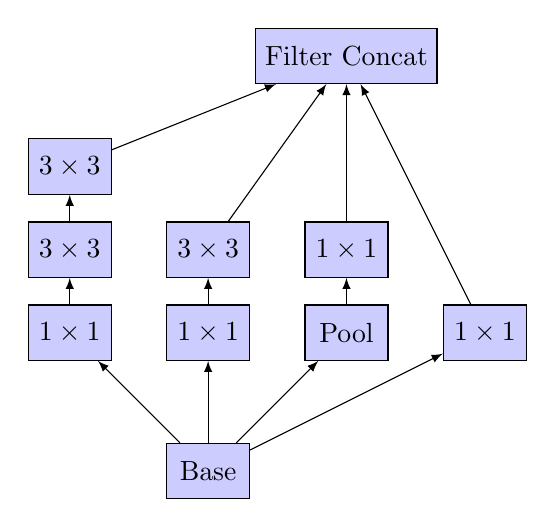
\begin{tikzpicture}[node distance=1.6cm]

    \node (concat) [block] {Filter Concat};

    \node (211) [block, below of=concat, node distance=7em] {$1\times1$};
    \node (233) [block, left of=211] {$3\times3$};
    \node (255) [block, left of=233] {$3\times3$};

    \node (333) [block, above of=255, node distance=3em] {$3\times3$};

    \node (pool) [block, below of=211, node distance=3em] {Pool};

    \node (1111) [block, left of=pool] {$1\times1$};
    \node (1112) [block, left of=1111] {$1\times1$};
    \node (1113) [block, right of=pool] {$1\times1$};

    \node (base) [block, below of=1111] {Base};

    
    \draw[arrow] (base) -- (1111);
    \draw[arrow] (base) -- (1112);
    \draw[arrow] (base) -- (pool);
    \draw[arrow] (base) -- (1113);

    \draw[arrow] (pool) -- (211);
    \draw[arrow] (1111) -- (233);
    \draw[arrow] (1112) -- (255);
    \draw[arrow] (1113) -- (concat);

    \draw[arrow] (255) -- (333);
    \draw[arrow] (333) -- (concat);
    \draw[arrow] (233) -- (concat);
    \draw[arrow] (211) -- (concat);

    

\end{tikzpicture}
    \captionof{figure}{Inception-Module (Version 2)}
    \label{fig:incept_modul2}
\end{minipage}

\newpage
\subsubsection{MobileNet}
Das \textit{MobileNet} \cite{howardMobileNetsEfficientConvolutional2017a}
wurde mit dem Ziel geschaffen, durch eine geringere 
Komplexität für mobile Endgeräte oder Embedded-Anwendungen 
geeignet zu sein.

Dafür wurden die üblichen \textit{Convolutional Layer}
durch sogenannten \textit{Depthwise Seperable 
Convolutions} ersetzt, welche die \Gls{faltung} in zwei separaten 
Schichten ausführt. Zuerst wird eine \textit{Depthwise  
Convolution} auf die drei Farbkanäle getrennt ausgeführt.
Anschließend führt eine \textit{pointwise convolution}
mit einem $1\times1$ Filter diese wieder zusammen.


In der zweiten Version des \textit{MobileNet}
\cite{sandlerMobileNetV2InvertedResiduals2019}
wurden die \textit{Depth-wise Separable Convolutions}
wie folgt abgeändert:

Zuerst wird eine $1\times1$ Convolution mit ReLU
Aktivierungsfunktion ausgeführt, gefolgt
von der \textit{Depthwise Convolution} und zum 
Schluss eine weitere $1\times1$ Convolution 
mit linearer Aktivierungsfunktion.


Des Weiteren soll wie beim \textit{ResNet} eine 
\textit{residual connection}, die Ein- und
Ausgabewert eines Blocks miteinander verbindet,
den Gradientenfluss unterstützen, wie in Abbildung 
\ref{fig:mobilenetv2} dargestellt ist.
\vspace{1cm}

\begin{figure}[H]
    \centering
    \includegraphics[width=0.7\textwidth]{mobilenet_v2.png}
    \caption{Residual block des MobilenetV2
    \cite{sandlerMobileNetV2InvertedResiduals2019}}
    \label{fig:mobilenetv2}
\end{figure}


%---------------- SUBSECTION: Obj Detection ----------------
\subsection{Objekterkennung}\label{subsec:objdet_det}

Neben der Information, was sich auf einem Bild befindet, 
soll bei der Objekterkennung zusätzlich herausgefunden werden, 
wo sich das erkannte Objekt in dem Bild befindet.
In Abbildung \ref{fig:class_vs_det} wird der Unterschied 
veranschaulicht. Im linken Bild (Klassifikation) 
reicht es aus, dass das Modell das Vorhandensein einer Katze
im Bild mit einer bestimmten Wahrscheinlichkeit vohersagen kann.
Im rechten Bild (Objekterkennung) soll das Modell,
in Form von Bounding-Boxen, zusätzlich eine Lokalisierung
der Objekte vornehmen.

\vspace{1cm}
\begin{minipage}{0.5\textwidth}
    \centering
    Klassifikation
\end{minipage}
\begin{minipage}{0.5\textwidth}
    \centering
    Objekterkennung
\end{minipage}
\begin{figure}[H]
    \centering
    \includegraphics[width=0.8\textwidth]{classification_detection.jpeg}
    \caption{Unterschied: Klassifikation und Objekterkennung 
    \cite{catDog}}
    \label{fig:class_vs_det}
\end{figure}
\vspace{1cm}

Dafür wird die \Gls{cnn}-Architektur so erweitert,
dass dem Modell für das Training neben den Klassen-Labels
auch die Koordinaten der Bounding-Boxen,
welche das Objekt umrahmen, mit übergeben werden.
Diese Koordinaten können mittels eines Regressionsverfahren
gelernt werden, wobei die geschätzten an die richtigen 
Koordinaten angenähert werden.

Bei den Verfahren zur Objekterkennung gibt es 
verschiedene Ansätze, die alle ein Basis-\Gls{cnn}
zur \textit{Feature Extraction} verwenden.
Die Lokalisierung findet über eine 
Vorschlagsgenerierung statt, welche aus 
Regionen im Inputbild besteht, die 
mit hoher Wahrscheinlichkeit ein Objekt enthalten.


%------------------- SECTION: Hardware ----------------------
\section{Neural Compute Stick 2}\label{ncs2}


Da das Training und die \Gls{inferenz} von Deep-Learning-Algorithmen
sehr rechenintensiv sind, werden entsprechend leistungsfähige 
Prozessoren benötigt. Dabei ist die Ausführung auf einer
\Gls{gpu} meist effizienter als auf einer \Gls{cpu}.

Anwendungen, die auf eingebetteten Systemen oder 
Einplatinencomputern wie dem \textit{Raspberry Pi} 
ausgeführt werden,
sind dementsprechend durch die Rechenleistung der Hardware
limitiert.

Eine Möglichkeit, diese Einschränkung zu umgehen,
besteht darin die Bilddaten für die Verarbeitung
 an eine Cloud zu senden, wo sie 
von einem leistungsstärkeren Rechner inferiert und 
anschließend wieder zurückgesendet werden.

Sollen die Daten, wie dies beim \textit{Edge Computing}
 der Fall ist, 
auf dem Anwendungsgerät direkt verarbeitet werden,
gibt es speziell für die \Gls{inferenz} von Deep-Learing-Algorithmen
geeignete Hardware.
Durch Fokus auf hohe Parallelität anstatt schneller Taktrate
bei den Berechnungen, können solche Prozessoren
Deep-Learning-spezifische Rechenoperationen, 
wie z.B. die Matrixmultiplikation, besonders effizient 
ausführen.

Die inferenzbeschleunigende Hardware kann dabei entweder
als eigenständiges \textit{\Gls{soc}}
System wie z.B. der \textit{Nvidia Jetson TX2} agieren, oder
in Verbindung mit einem \textit{Host PC}, wie der in der Arbeit 
verwendete \textit{Neural Compute Stick 2} (NCS2) von
\textit{Intel}.

Der in Abbildung \ref{fig:ncs2} gezeigte NCS2
verwendet für die \Gls{inferenz} eine
\textit{Movidius Myriad X} \textit{\Gls{vpu}},
welche in Abbildung \ref{fig:myriad} schematisch 
dargestellt ist.

Diese besteht aus der Neural Compute Engine 
zur beschleunigten Berechnung Neuronaler Netze,
einem Bildbeschleuniger, 16 SHAVE Prozessoren, einem 
Bildsignalprozessor sowie einem RISC CPU Core. 
\cite{haussermann}

\vspace{1cm}
\begin{minipage}{0.4\textwidth}
    \centering
    \includegraphics[width=\textwidth]{ncs2_top.jpg}
    \captionof{figure}{Neural Compute Stick 2 \cite{ncs2}}
    \label{fig:ncs2}
\end{minipage}
\begin{minipage}{0.6\textwidth}
    \centering
    \includegraphics[width=\textwidth]{myriad.png}
    \captionof{figure}{Movidius Myriad X
    \cite{myriad}}
    \label{fig:myriad}
\end{minipage}


\subsection{OpenVino Toolkit}

Zur Ausführung der \Gls{inferenz} eines trainierten Deep-Learing-Modells
auf dem NCS2 wird das Toolkit 
\textit{OpenVino} von Intel verwendet.
Dabei handelt es sich um eine Software Plattform
zur Optimierung und \Gls{inferenz} 
von \Gls{cnn}-basierten Modellen auf verschiedener
Intel-Hardware.

Für die Modelle wird dabei ein eigenes Dateiformat verwendet, 
die \textit{Intermediate Representation} (IR),
welche die Struktur des Modells 
in einer Xml-Datei und die trainierten Gewichte in 
einer Binärdatei definiert.
Mit dem \textit{Model Optimizer} des Toolkits
können Modelle, die in den \Glspl{framework}
 \textit{TensorFlow,
Caffe, ONNX, Kaldi,} oder \textit{MXNET} trainiert wurden, 
in das IR-Format konvertiert werden.


Um diese Modelle dann auf die entsprechende Hardware
zu laden und anwendbar zu machen, wird die auch
in \textit{OpenVino} enthaltene
\textit{InferenceEngine} verwendet.
Diese bietet eine \Gls{api}, mit der aus der Anwendung
heraus, in den Programmiersprachen C++ oder Python,
auf die Funktionen der 
\textit{InferenceEngine} zugegriffen werden kann.


In Abbildung \ref{fig:openvinoflow} ist der Workflow mit 
\textit{Openvino} dargestellt, der das Training eines
Deep-Learning-Modells mit der Implementierung
einer Nutzeranwendung verbindet


\vspace{1cm}
\begin{figure}[H]
    \centering
    \def\svgwidth{0.8\textwidth}
    \input{Bilder/open_vino_workflow_neu.pdf_tex}
    \caption{OpenVino Workflow orientiert an 
    \cite{openvinoflow}}
    \label{fig:openvinoflow}
\end{figure}
